%===================================================================================
% JORNADA CIENTÍFICA ESTUDIANTIL - MATCOM, UH
%===================================================================================
% Esta plantilla ha sido diseñada para ser usada en los artículos de la
% Jornada Científica Estudiantil de MatCom.
%
% Por favor, siga las instrucciones de esta plantilla y rellene en las secciones
% correspondientes.
%
% NOTA: Necesitará el archivo 'jcematcom.sty' en la misma carpeta donde esté este
%       archivo para poder utilizar esta plantila.
%===================================================================================



%===================================================================================
% PREÁMBULO
%-----------------------------------------------------------------------------------
\documentclass[a4paper,10pt,twocolumn]{article}

%===================================================================================
% Paquetes
%-----------------------------------------------------------------------------------
\usepackage{amsmath}
\usepackage{amsfonts}
\usepackage{amssymb}
\usepackage{jcematcom}
\usepackage[utf8]{inputenc}
\usepackage{listings}
\usepackage[pdftex]{hyperref}
\usepackage{caption}
\usepackage{subcaption}
%-----------------------------------------------------------------------------------
% Configuración
%-----------------------------------------------------------------------------------
\hypersetup{colorlinks,%
	    citecolor=black,%
	    filecolor=black,%
	    linkcolor=black,%
	    urlcolor=blue}

%===================================================================================

%===================================================================================
% Presentacion
%-----------------------------------------------------------------------------------
% Título
%-----------------------------------------------------------------------------------
\title{Patrón cualitativo de trayectorias para el movimiento radial del sistema Tierra-Luna}

%===================================================================================
% DOCUMENTO
%-----------------------------------------------------------------------------------
\begin{document}

%-----------------------------------------------------------------------------------
% NO BORRAR ESTA LINEA!
%-----------------------------------------------------------------------------------
\twocolumn[
%-----------------------------------------------------------------------------------

\maketitle

%===================================================================================
% Resumen y Abstract
%-----------------------------------------------------------------------------------
\selectlanguage{spanish} % Para producir el documento en Español

%-----------------------------------------------------------------------------------
% Resumen en Español
%-----------------------------------------------------------------------------------
\begin{abstract}

	Interpretación de las trayectorias para la ecuación del movimiento radial en el sistema Tierra-Luna. Revela un patrón cualitativo gobernado por una estabilidad regional separada por fronteras de alta sensibilidad. El sistema se caracteriza por dos regiones de atracción claramente definidas —una hacia la Tierra y otra hacia la Luna—, entre las cuales se establece una frontera crítica en el punto de equilibrio gravitatorio. La mayor parte del espacio muestra un comportamiento estable, con trayectorias de pendiente casi horizontal que denotan una variación mínima de la velocidad. Sin embargo, este régimen estable se interrumpe en dos umbrales de destino clave: la vecindad del eje de velocidad cero y, de manera más crítica, la región cercana al equilibrio. En estos umbrales, la más mínima perturbación en las condiciones iniciales determina irreversiblemente el destino del cuerpo, definiendo así un sistema altamente sensible donde dominan las transiciones abruptas sobre las variaciones suaves.

\end{abstract}

%-----------------------------------------------------------------------------------
% English Abstract
%-----------------------------------------------------------------------------------

\vspace{0.5cm}

\begin{enabstract}

  Interpretation of Trajectories for the Radial Motion Equation in the Earth-Moon System. The analysis reveals a qualitative pattern governed by regional stability separated by boundaries of high sensitivity. The system is characterized by two clearly defined regions of attraction—one towards the Earth and another towards the Moon—between which a critical frontier is established at the gravitational equilibrium point. Most of the phase space exhibits stable behavior, with trajectories of near-horizontal slope indicating minimal variation in velocity. However, this stable regime is interrupted at two key destiny thresholds: the vicinity of the zero-velocity axis and, more critically, the region near the equilibrium point. At these thresholds, the slightest perturbation in the initial conditions irreversibly determines the body's fate, thus defining a highly sensitive system where abrupt transitions dominate over smooth variations.

\end{enabstract}


%-----------------------------------------------------------------------------------
% NO BORRAR ESTAS LINEAS!
%-----------------------------------------------------------------------------------
\vspace{0.8cm} ]
%-----------------------------------------------------------------------------------


%===================================================================================

%===================================================================================
% Resumen Extendido
%-----------------------------------------------------------------------------------
\section{Resumen Extendido}\label{sec:intro}
%-----------------------------------------------------------------------------------
El estudio del movimiento de un cuerpo bajo la influencia gravitatoria combinada de la Tierra y la Luna permite comprender fenómenos de estabilidad, escape y colisión en sistemas de dos cuerpos. A partir de un modelo unidimensional del movimiento radial, se analiza el comportamiento cualitativo del sistema mediante el trazado del campo de isoclinas asociado a la ecuación diferencial del movimiento, con el objetivo de identificar regiones de estabilidad o inestabilidad, así como la sensibilidad del sistema ante perturbaciones iniciales.

Se considera la ecuación diferencial que modela el movimiento radial en el sistema Tierra–Luna,

$f(r,v)=\frac{\frac{-GM_e}{r^2}+\frac{GM_m}{(S-r)^2}}{v}$ donde $M_e$ y $M_m$ son las masas de la Tierra y la Luna respectivamente y S la distancia entre ambos cuerpos. A partir de esta expresión se genera el campo de isoclinas (Fig. 1), representando las pendientes $\frac{dv}{dr}$ en cada punto del plano. 


El patrón cualitativo de las trayectorias muestra un comportamiento dominado por dos regiones de atracción gravitatoria determinadas por cada uno de los términos de la ecuación: uno cerca de la Tierra, y otra cerca de la Luna.

  \begin{figure}
    \centering
    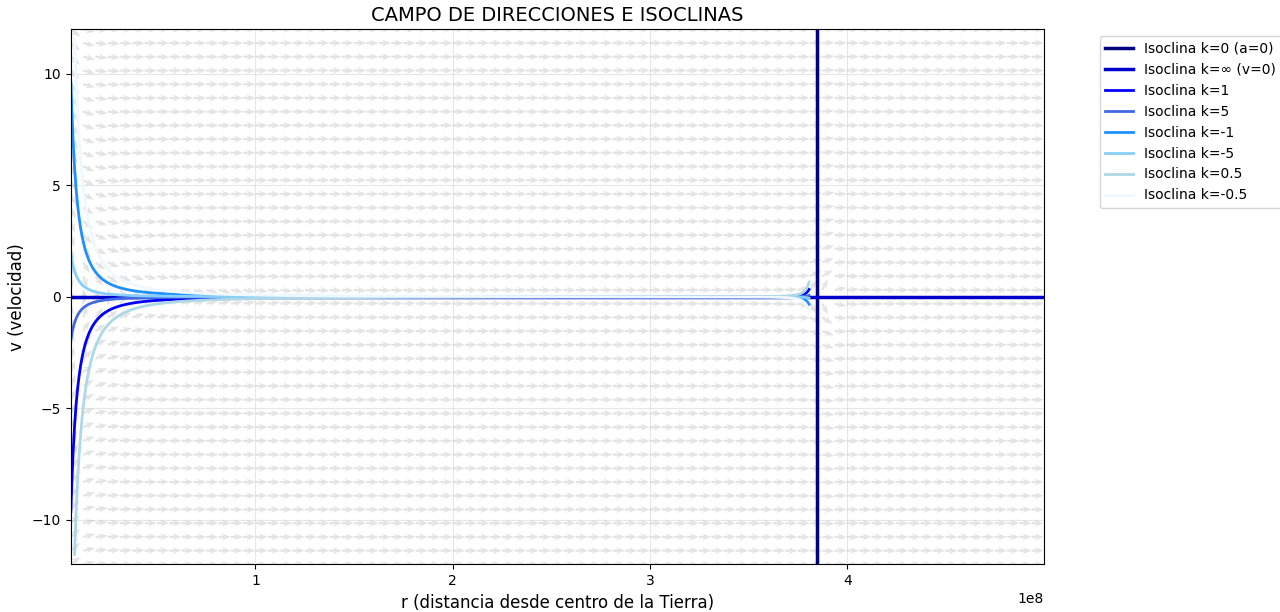
\includegraphics[width=1\linewidth]{isoclines.png}
    \caption{Campo de isoclinas correspondiente al movimiento radial en el sistema Tierra–Luna.}
    \label{fig:placeholder}
\end{figure}
%-----------------------------------------------------------------------------------
A partir del campo de direcciones, pueden distinguirse tres zonas de gran relevancia:
\begin{enumerate}
	\item Eje $v$: Dado que el término $\frac{1}{v}$ en la ecuación se dispara cuando $v\approx$0, la región tiene un comportamiento inestable, es decir, variaciones en $v$ generan cambios bruscos de pendiente. Para $v>0$ las pendientes son negativas y para $v<0$ positivas, lo que corresponde a puntos de retorno o colisión donde la dinámica del sistema cambia abruptamente.
	\item Cercano al eje $r$: Corresponde a la zona de influencia gravitatoria terrestre. Posee una alta sensibilidad respecto a $v$, observándose en los cambios bruscos de la dirección de las pendientes.
	\item Línea vertical $r=r_e:$ En el punto de equilibrio, donde las atracciones de la Tierra y la Luna se compensan, el sistema actúa como un umbral energético. Si la velocidad inicial es apenas positiva, se desplaza hacia la Luna; si es apenas negativa, regresa hacia la Tierra. Este comportamiento refleja una inestabilidad inherente a las variaciones de $v$.
    
    En el resto del campo, las pendientes son prácticamente horizontales, lo que indica que la variación de $v$ respecto a $r$ es mínima. En estas regiones, la aceleración neta es casi nula y se mantiene la velocidad con poca variación, reflejando un comportamiento estable. 

    Podemos corroborar estas observaciones cualitativas a partir de las \textbf{isoclinas} del sistema. Para ello, se trazan las curvas correspondientes a las pendientes $k = 1$, $k = -1$, $k = 5$, $k = -5$, $k = 0.5$, $k = -0.5$, $k = 0$ y pendiente infinita. Con el fin de facilitar el análisis, se dividen en \textbf{isoclinas positivas y negativas}, dejando como casos particulares a $k = 0$ y a la pendiente infinita. 
    Este análisis confirma los hallazgos del campo de pendientes: las \textbf{isoclinas positivas} aparecen principalmente cerca de la \textbf{influencia lunar}, donde la aceleración neta es positiva, favoreciendo un aumento de la velocidad; las \textbf{negativas} dominan en la \textbf{región terrestre}, donde la aceleración es negativa; las isoclinas $k = 0$ y la de pendiente infinita representan, respectivamente, las condiciones $v = 0$ y $a = 0$, delimitando \textbf{transiciones entre ambos regímenes}. Finalmente, en las proximidades del punto de equilibrio, las isoclinas se agrupan densamente y cambian de signo con rapidez, corroborando visualmente la alta sensibilidad y la inestabilidad que se infirió inicialmente a partir del campo de direcciones.
    
\end{enumerate}

\label{end}

\end{document}

%===================================================================================
